\documentclass{article}
\usepackage{graphicx}
\usepackage{url}

\begin{document}
\title{Aaron McKay - Research and Background}
\author{Aaron McKay}
\maketitle

% Your content from first assignment
\section{About Me}
I am a 2nd year PhD student at UCCS.  I haven't yet published a paper but I'm working on it.  My area of research I think is one of the most challenging in all of cybersecurity, Cyber Risk Quantification (CRQ).  Its taken me some time to figure out how this problem is best approached and I think the answer lies in a deep classification and analysis of the interactions of Attackers and Defenders. There may be several derivations from this interaction, but since my attention is on cyber risk quantification, my focus is on "Susceptibility" of Systems and Users not only as a metric but as a factor to be used upstream the CRQ calculations.
\begin{figure}[h]
    \centering
    
\includegraphics[width=0.5\textwidth]{images/Oh_Yeah.jpg}
    \caption{Oh Yeah}
    \label{fig:oh-yeah}
\end{figure}

\section{Research Code Experience}
\subsection{Repository Used}
I explored the Netflix-Skunkworks RiskQuant repository 
(\url{https://github.com/Netflix-Skunkworks/riskquant}). While attempting to use 
the full repository, I encountered compatibility issues with the required dependencies. 
This led me to implement a simplified version of the risk quantification concepts 
to demonstrate the core principles.

\begin{figure}[h]
    \centering
    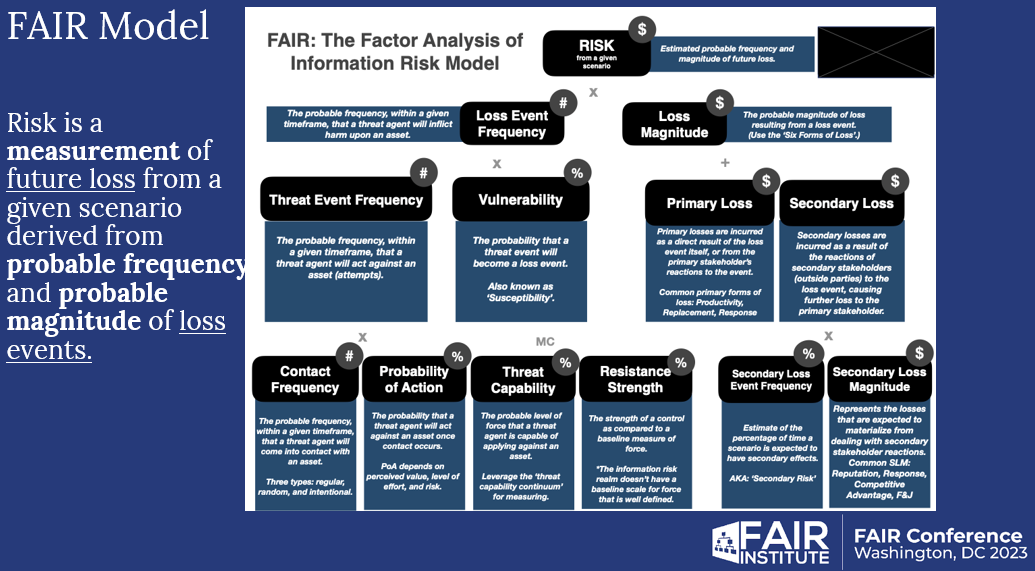
\includegraphics[width=\textwidth]{images/fair_model.png}
    \caption{FAIR (Factor Analysis of Information Risk) Model presented at FAIR Conference 2023, Washington, DC. The FAIR model is a popular implementation of CRQ.
    Credit: Jon Baker (Co-founder \& Director, Center for Threat-Informed Defense), 
    Arvin Bansal (vCISO, Fortune500), and Vidit Baxi (Co-founder \& CISO, Safe Security)}
    \label{fig:fair-model}
\end{figure}

\subsection{Testing Experience}
I created a basic risk quantification model that implements Monte Carlo simulation 
to estimate potential losses from cyber incidents. The model takes into account:
\begin{itemize}
    \item Minimum and maximum potential losses (\$100,000 to \$1,000,000)
    \item Annual probability of occurrence (10\%)
    \item 10,000 simulation iterations for statistical significance
\end{itemize}

The simulation provides insights into potential cyber incident costs, including average 
annual loss, maximum potential loss, and the 90th percentile loss value.

\subsection{Output Examples}
\begin{verbatim}
Risk Analysis for Data Breach Scenario:
Average Annual Loss: $52,624.65
Maximum Potential Loss: $999,737.69
90th Percentile Loss: $0.00
\end{verbatim}

\subsection{Analysis}
The results show an average annual loss of about \$52,600, which aligns with the 
10\% probability of an incident occurring. The maximum potential loss approaches 
the upper limit of \$1,000,000, demonstrating the model's ability to capture 
worst-case scenarios. The 90th percentile being \$0 indicates that in most 
simulation runs (over 90\%), no loss occurred, which is consistent with the 
low probability of occurrence.

\section{Merge Conflict and Permission Resolution}
During this assignment, I encountered two significant challenges that required resolution:

\subsection{Repository Permission Issues}
Initially, I was unable to push my changes to the repository due to permission restrictions. I attempted several approaches:
\begin{enumerate}
    \item First tried pushing directly using HTTPS protocol (received 403 error)
    \item Attempted using SSH authentication
    \item Created a fork of the repository as a backup
    \item Generated a patch file (mckay-changes.patch) to preserve my changes
    \item Finally resolved when Dr. Boult granted proper repository access
\end{enumerate}

\subsection{Merge Conflicts}
After gaining proper access, I encountered merge conflicts when trying to merge upstream/main into my branch. 
The conflicts involved two files (cardenas.tex and jcastanonremy.tex) that were deleted in my branch 
but modified in upstream/main. I resolved these conflicts by:
\begin{enumerate}
    \item First checking the status using git status to understand the nature of the conflicts
    \item Using git rm --cached to remove the conflicting files from Git tracking
    \item Committing the resolution with an appropriate commit message
    \item Cleaning up the working directory by removing the untracked files
    \item Successfully completing the merge afterward
\end{enumerate}

This experience helped me understand both the importance of proper repository permissions and 
how to handle conflicts between different branches in a Git repository. It demonstrated 
real-world scenarios of collaboration challenges and their solutions.

\section{Questions and Answers}
% This section will be used later for Q&A

\end{document}

